\section{Testování naučeného modelu}
Pro testování modelu chceme generovat nové vzorky – toho lze dosáhnout použitím hodnot ze $z \sim \mathcal{N}$ jako vstup pro dekodér.
Jedná se tedy vlastně o odstranění enkodéru (včetně operací násobení a sčítání, které by jinak měnily rozdělení pravděpodobnosti $z$). \cite{Doersch2021}

Schéma této jednoduché sítě prezentuje \autoref{fig:vae_sample}.

\begin{figure}[H]
    \centering
    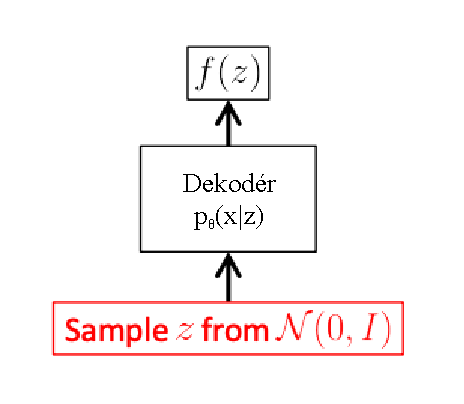
\includegraphics{figures/vae_sample.pdf}
    \caption{Test-time schéma variačního autoenkodéru, které umožňuje generovat nové vzorky. Jelikož k vygenerování nového vzorku není potřeba enkodér, je vazba na něj jednoduše smazána (oproti sítí, kterou zachycuje \autoref{fig:vae_backpropagation}). Schéma a interpretace převzato z \cite{Doersch2021}.}
    \label{fig:vae_sample}
\end{figure}

Chceme-li vyhodnotit pravděpodobnost vygenerování konkrétního vzorku z naučeného modelu, jedná se o efektivně neřešitelný problém (tento problém adresuje architektura tzv. Conditional variačních autoenkodérů, viz \autoref{sec:cvae}).